% !TEX root = ./correctness-deciders.tex
\newpage
\section{Finite automata reduction}\label{sec:finite-automata-reduction}

\subsection{Method overview}\label{far-overview}

The core idea of the method presented in this section is to find, for a given Turing machine, a regular language that contains the set of the machine's eventually-halting configurations. Then, provided that the all-0 configuration is not in the regular language, we know that the machine does not halt.

A dual idea has been explored by other authors under the name Closed Tape Languages (CTL) as described in S. Ligocki's blog \cite{ShawnCTL} and credited to H. Marxen in collaboration with J. Buntrock.
The CTL technique for proving a Turing machine doesn't halt is to exhibit a set $C$ of configurations such that:

\begin{enumerate}
  \item $C$ contains the all-0 initial configuration\footnote{
          Criteria 1--2 give a strict definition; in \cite{ShawnCTL}, $C$ only needs to contain some descendant of the initial configuration and some descendant of the successor to each $c\in C$.
          In that case, the set of ancestor configurations to those in $C$ meets the strict definition.
        }
  \item $C$ is \textit{closed} under transitions: for any $c \in C$, the configuration one step later belongs to $C$\addtocounter{footnote}{-1}\addtocounter{Hfootnote}{-1}\footnotemark
  \item $C$ does not contain any halting configuration
\end{enumerate}


If such a set $C$ exists then the machine does not halt.
The CTL approach has proven to be practical and powerful when we search for $C$ among regular languages \cite{ShawnCTL} \cite{BruteforceCTL}.

Here, we develop an original \textit{co-CTL} technique\footnote{By co-CTL we mean a set whose complement is a CTL, characterized by closure criteria inverse---or equivalently converse---to 1--3. In other words, a co-CTL contains all halting configurations, any configuration which can \emph{precede} any member configuration by one TM transition, and not the initial configuration.}, based on the algebraic description of Nondeterministic Finite Automata (NFA), for finding a regular language which contains a machine's eventually halting configurations (in general a superset).

One important aspect of the technique is that, given a Turing machine and its constructed NFA---if found---it is a computationally simple task to verify that the NFA's language does indeed recognise all eventually-halting configurations of the machine.


\usetikzlibrary {automata, positioning}

\begin{figure}
  \begin{center}
    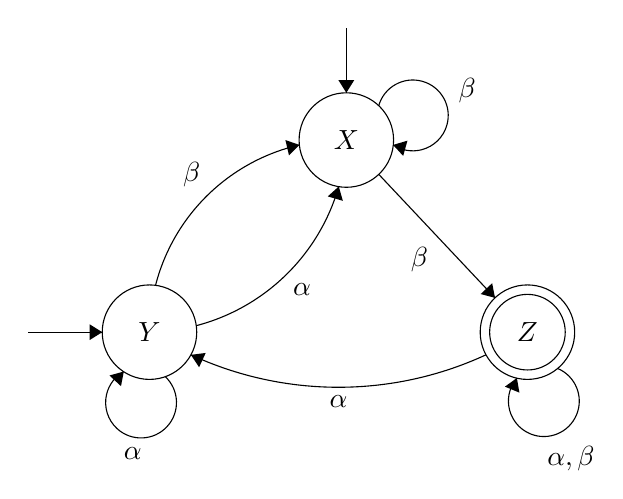
\begin{tikzpicture}[scale=0.2]
      \tikzstyle{every node}+=[inner sep=0pt]
      \draw [black] (32.4,-20.7) circle (3);
      \draw (32.4,-20.7) node {$X$};
      \draw [black] (19.9,-32.9) circle (3);
      \draw (19.9,-32.9) node {$Y$};
      \draw [black] (43.9,-32.9) circle (3);
      \draw (43.9,-32.9) node {$Z$};
      \draw [black] (43.9,-32.9) circle (2.4);
      \draw [black] (12.2,-32.9) -- (16.9,-32.9);
      \fill [black] (16.9,-32.9) -- (16.1,-32.4) -- (16.1,-33.4);
      \draw [black] (32.4,-13.6) -- (32.4,-17.7);
      \fill [black] (32.4,-17.7) -- (32.9,-16.9) -- (31.9,-16.9);
      \draw [black] (31.917,-23.654) arc (-16.01031:-75.38142:12.771);
      \fill [black] (31.92,-23.65) -- (31.22,-24.28) -- (32.18,-24.56);
      \draw (29.58,-29.75) node [below] {$\alpha$};
      \draw [black] (20.894,-35.718) arc (47.15723:-240.84277:2.25);
      \draw (18.84,-40.19) node [below] {$\alpha$};
      \fill [black] (18.27,-35.4) -- (17.36,-35.65) -- (18.09,-36.33);
      \draw [black] (20.283,-29.932) arc (165.64786:102.96041:12.277);
      \fill [black] (29.42,-21.01) -- (28.53,-20.7) -- (28.76,-21.68);
      \draw (22.58,-23.71) node [above] {$\beta$};
      \draw [black] (34.46,-22.88) -- (41.84,-30.72);
      \fill [black] (41.84,-30.72) -- (41.66,-29.79) -- (40.93,-30.48);
      \draw (37.62,-28.27) node [left] {$\beta$};
      \draw [black] (34.454,-18.529) arc (164.32314:-123.67686:2.25);
      \draw (39.49,-17.55) node [right] {$\beta$};
      \fill [black] (35.37,-21.01) -- (36.01,-21.71) -- (36.28,-20.74);
      \draw [black] (45.807,-35.201) arc (67.3925:-220.6075:2.25);
      \draw (46.66,-40.1) node [below] {$\alpha,\beta$};
      \fill [black] (43.23,-35.81) -- (42.47,-36.36) -- (43.39,-36.74);
      \draw [black] (41.27,-34.338) arc (-65.18014:-114.81986:22.321);
      \fill [black] (22.53,-34.34) -- (23.05,-35.13) -- (23.47,-34.22);
      \draw (31.9,-36.9) node [below] {$\alpha$};
    \end{tikzpicture}
  \end{center}
  \caption{Example Nondeterministic Finite Automaton (NFA) with 3 states X,Y and Z, alphabet $\mathcal{A} = \{\alpha,\beta\}$, initial states X and Y, and accepting state Z. The linear-algebra representation of this NFA is given in Example~\ref{ex:nfa}. Example accepted words are: $\beta$, $\alpha\beta$, $\alpha\alpha\beta\beta$. Example rejected words are: $\alpha$, $\alpha\alpha$, $\alpha\alpha\alpha$.}\label{fig:example_nfa}
\end{figure}

\begin{figure}

  % \begin{subfigure}[m]{0.13\textwidth}
  %   \centering
  %   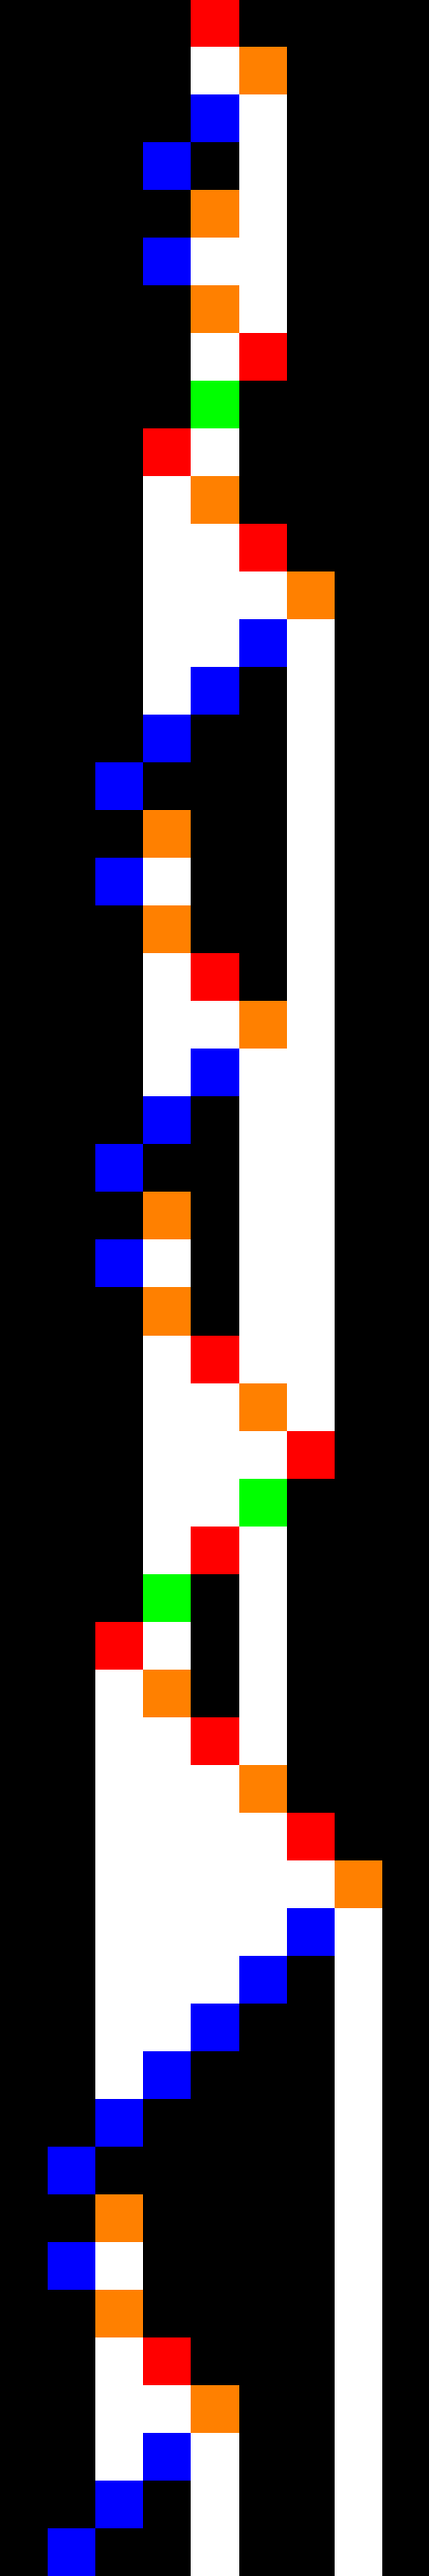
\includegraphics[width=\textwidth]{space-time-diagrams/finite-automata-reduction-counter4.pdf}
  %   \caption{First few descendants of \tss{a 4-state TM's}{the initial all-0 configuration for the machine given in (\ref{fig:far_transitions})}.}
  %   \label{fig:far_spacetime}
  % \end{subfigure}
  % \hfill
  % \parbox{0.2\textwidth}{
  %   \begin{subfigure}[t]{0.22\textwidth}
  %     \centering
  %     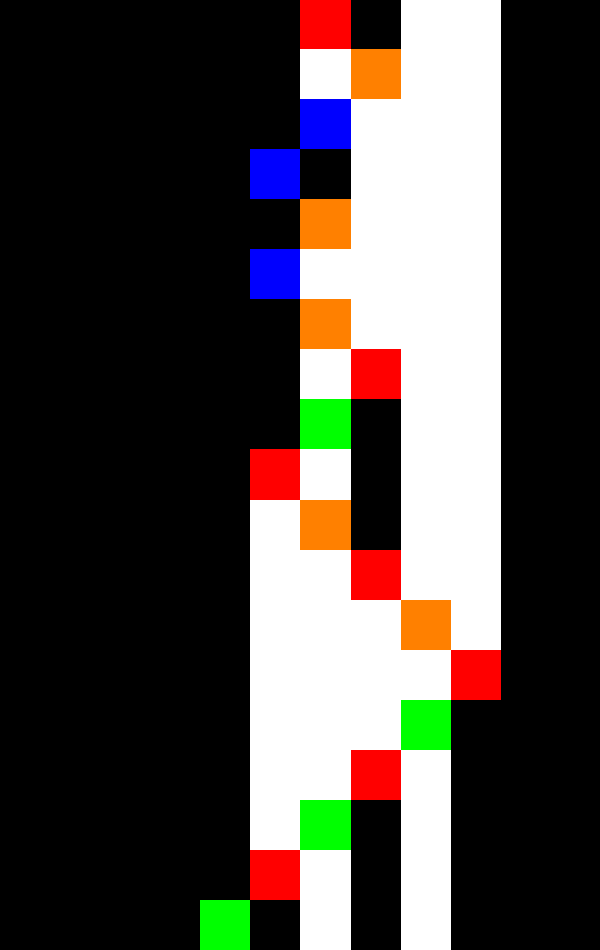
\includegraphics[width=\textwidth]{space-time-diagrams/finite-automata-reduction-counter4-halt.pdf}
  %     \caption{\tss{The same TM halts in these configurations.}{Some  eventually-halting successive configurations of the machine given in (\ref{fig:far_transitions}): the machine halts after 18 steps by reading a 0 in state D.}}
  %     \label{fig:far_spacetime_halt}
  %   \end{subfigure}
  %   \vspace{0.23\textheight}

  %   \begin{subfigure}[t]{0.2\textwidth}
  %     \centering
  %     \begin{tabular}{lll}
  %                             & 0                       & 1                       \\
  %       \textcolor{colorA}{A} & 1R\textcolor{colorB}{B} & 0L\textcolor{colorD}{D} \\
  %       \textcolor{colorB}{B} & 1L\textcolor{colorC}{C} & 1R\textcolor{colorA}{A} \\
  %       \textcolor{colorC}{C} & 0R\textcolor{colorB}{B} & 0L\textcolor{colorC}{C} \\
  %       \textcolor{colorD}{D} & - - -                   & 1L\textcolor{colorA}{A} \\
  %     \end{tabular}
  %     \caption{Transition table.}
  %     \label{fig:far_transitions}
  %   \end{subfigure}
  % }
  % \hfill
  % \begin{subfigure}[m]{0.62\textwidth}
  %   \begin{tikzpicture}[shorten >=1pt]
  %     \node[state,initial above] (0) at (-2, 2) {0};
  %     \node[state]           (1) at (-2, -2) {1};
  %     \node[state,accepting] (H) at (2, 4) {$\bot$};
  %     \node[state]           (0A) at (0, 2) {0A};
  %     \node[state,accepting] (0D) at (4, 2) {0D};
  %     \node[state]           (0B) at (2, 0) {0B};
  %     \node[state]           (0C) at (4, 0) {0C};
  %     \node[state]           (1C) at (2, -2.5) {1C};
  %     \node[state]           (1B) at (0, -4) {1B};
  %     \node[state]           (1A) at (4, -4) {1A};
  %     \node[state,accepting] (1D) at (5.5, -2) {1D};

  %     \path[->]  (0)  edge [loop right]       node {$0$} (0)
  %     edge                    node [right] {$1$} (1)
  %     (1)  edge [bend left=15]     node [above left] {$0|1$} (0)
  %     (0A) edge                    node [right] {$0$} (1B)
  %     edge                    node [above,rotate=60] {$1$} (H)
  %     (0C) edge                    node [above] {$0$} (0B)
  %     edge                    node [right] {$1$} (1A)
  %     (0D) edge                    node [above,rotate=300] {$0$} (H)
  %     edge                    node [above] {$1$} (0A)
  %     edge [bend left]        node [left] {$1$} (1A)
  %     (1A) edge                    node [above] {$1$} (1B)
  %     (1A) edge [bend right=15]    node [above,rotate=300] {$0|1$} (0B)
  %     (0B) edge [bend right=5]     node [above,rotate=300] {$0|1$} (1A)
  %     (1B) edge                    node [above right,rotate=60] {$0$} (0B)
  %     edge [loop left]        node {$0$} (1B)
  %     edge [bend left]        node [right] {$1$} (0A)
  %     (1C) edge                    node [above right,rotate=270] {$0|1$} (0B)
  %     (1D) edge [bend right=48]    node [below,rotate=300] {$0|1$} (H)
  %     (H)  edge [loop above]       node {$0|1$} (H)
  %     (0)  edge [dotted,bend left] node {\textcolor{colorA}{A}} (0A)
  %     edge [dotted]           node [left] {\textcolor{colorB}{B}} (0B)
  %     edge [dotted]           node {\textcolor{colorC}{C}} (0C)
  %     edge [dotted,bend left] node [right] {\textcolor{colorD}{D}} (0D)
  %     (1)  edge [dotted]           node {\textcolor{colorB}{B}} (1B)
  %     edge [dotted]           node {\textcolor{colorA}{A}} (1A)
  %     edge [dotted]           node [left] {\textcolor{colorC}{C}} (1C)
  %     edge [dotted]           node [left] {\textcolor{colorD}{D}} (1D);
  %   \end{tikzpicture}
  %   \caption[Caption for figure]{Diagram of a Nondeterministic Finite Automaton\ts{, constructed using the direct FAR algorithm (Section~\ref{far-algo-direct}),} recognizing at least all \tss{rows of (\ref{fig:far_spacetime_halt}) but none of (\ref{fig:far_spacetime})}{eventually-halting configurations of the machine given in (\ref{fig:far_transitions}). For instance, it recognises all rows of (\ref{fig:far_spacetime_halt}). However, it recognises no rows of (\ref{fig:far_spacetime}), hence the machine does not halt from the all-0 configuration.}}
  %   \label{fig:far_nfa}
  % \end{subfigure}
  % \bigskip

  % \begin{subfigure}{\textwidth}
  %   \usetikzlibrary{chains,fit,shapes}
  %   \begin{tikzpicture}
  %     \tikzstyle{tmtape}=[draw,minimum size=15mm]
  %     \tikzstyle{tmhead}=[arrow box,draw,minimum size=10mm,arrow box arrows={east:3mm, west:3mm},minimum height=5mm]
  %     \tikzstyle{fastate}=[draw,minimum size=10mm,minimum height=64pt]
  %     \begin{scope}[start chain=1 going right,node distance=0]
  %       \node [on chain=1,tmtape,draw=none] (--) {Configuration: \dots};
  %       \node [on chain=1,tmtape] (-2) {\textbf{0}};
  %       \node [on chain=1,tmtape] (-1) {\textbf{0}};
  %       \node [on chain=1,tmtape] (-0) {\textbf{0}};
  %       \node [on chain=1,tmtape] (+1) {\textbf{0}};
  %       \node [on chain=1,tmtape] (+2) {\textbf{1}};
  %       \node [on chain=1,tmtape] (+3) {\textbf{1}};
  %       \node [on chain=1,tmtape] (+4) {\textbf{0}};
  %       \node [on chain=1,tmtape] (+5) {\textbf{0}};
  %       \node [on chain=1,tmtape,draw=none] (++) {$\dots$};
  %     \end{scope}
  %     \node [tmhead,yshift=-3mm] at (-0.south) (+0) {\textcolor{colorA}{A}};

  %     \begin{scope}[start chain=2 going right,node distance=5mm]
  %       \node [on chain=2,fastate,draw=none,below=of --,xshift=-.5cm,yshift=-5mm] (a--) {Scan: \dots};
  %       \node [on chain=2,fastate] (a-2) {0};
  %       \node [on chain=2,fastate] (a-1) {0};
  %       \node [on chain=2,fastate,minimum height=24pt,yshift=-18pt] (a-0) {0A};
  %       \node [above=of a-0,fastate,minimum height=24pt] (a+0) {1B};
  %       \node [on chain=2,fastate,yshift=18pt] (a+1) {$\begin{aligned}&\textrm{0B}\\|&\textrm{1B}\end{aligned}$};
  %       \node [on chain=2,fastate] (a+2) {$\begin{aligned}&\textrm{0A}\\|&\textrm{1A}\end{aligned}$};
  %       \node [on chain=2,fastate] (a+3) {$\begin{aligned}&\bot\\|&\textrm{0B}\\|&\textrm{1B}\end{aligned}$};
  %       \node [on chain=2,fastate] (a+4) {$\begin{aligned}&\bot\\|&\textrm{0B}\\|&\textrm{1A}\\|&\textrm{1B}\end{aligned}$};
  %       \node [on chain=2,fastate] (a+5) {$\begin{aligned}&\bot\\|&\textrm{0B}\\|&\textrm{1A}\\|&\textrm{1B}\end{aligned}$};
  %       \node [on chain=2,fastate,draw=none] (a++) {$\dots$};
  %     \end{scope}

  %     \path (a--) edge node [above] {$\boldsymbol{0}$} (a-2)
  %     (a-2) edge node [above] {\textbf{0}} (a-1)
  %     (a-1) edge node [above] {\textbf{A}} (a-0)
  %     (a-0) edge node [right] {\textbf{0}} (a+0)
  %     (a+0) edge node [above] {\textbf{0}} (a+1)
  %     (a+1) edge node [above] {\textbf{1}} (a+2)
  %     (a+2) edge node [above] {\textbf{1}} (a+3)
  %     (a+3) edge node [above] {\textbf{0}} (a+4)
  %     (a+4) edge node [above] {\textbf{0}} (a+5)
  %     (a+5) edge                    (a++);
  %   \end{tikzpicture}
  %   \caption{\tss{An NFA with transitions (\ref{fig:far_nfa}), scanning the top row of (\ref{fig:far_spacetime_halt}), stays in ``accepted'' state
  %       $\bot|\textrm{0B}|\textrm{1A}|\textrm{1B}$.}{oo}}
  %   \label{fig:far_scan}
  % \end{subfigure}
  \centering
  \includegraphics*[scale=0.6]{FAR.pdf}

  \caption{\small A Nondeterministic Finite Automaton, used as follows to decide a 4-state Turing machine\protect\footnotemark:
    (a) Space-time diagram showing the first few descendants of the all-0 configuration for the machine. The machine actually runs forever from the all-0 configuration, adopting a ``counting'' behavior.
    (b) The TM halts in 18 steps from a different configuration; these 18 rows depict \emph{eventually-halting} configurations.
    (c) Transition table for the TM.
    (d) A Nondeterministic Finite Automaton, constructed using the direct FAR algorithm (Section~\ref{far-algo-direct}), that recognises at least all eventually-halting configurations of the machine. For instance, inputting the top row of (b), encoded as word \texttt{000A01100} (see Definition~\ref{def:wordc}), the NFA transitions by reading each successive symbol of the input, through NFA states: 0, 0, 0A, 1B, \{0B, 1B\}, \{0A, 1A\}, \{$\bot$, 0B, 1B\}, \{$\bot$, 0B, 1A, 1B\} and finally \{$\bot$, 0B, 1A, 1B\}. Since NFA state $\bot$ is accepting (doubly circled in (d)), the NFA accepts \texttt{000A01100}, classifying this configuration as potentially eventually-halting. However, the NFA does not accept input \texttt{A0}, which corresponds to the all-0 configuration, hence this TM cannot halt from there.}



  \label{fig:finite-automata-reduction}
\end{figure}

\footnotetext{\url{https://bbchallenge.org/1RB0LD_1LC1RA_0RB0LC_---1LA}}

\subsection{Potential-halt-recognizing automata}
\newcommand{\M}{\mathcal{M}}
\newcommand{\T}{^T}
\newcommand{\row}{\text{row}}
\label{far-defs-recognizer}
For a given Turing machine, we aim at building an NFA that recognises at least all eventually-halting configurations. In other words, the NFA recognises configurations that \textit{potentially} eventually halt, which is why we call the NFA \textit{potential-halt-recognizing}. Importantly, if the NFA does not recognise the all-0 initial configuration then we know that the Turing machine does not halt from it.


Let's first recall how Nondeterministic Finite Automta (\textbf{NFA}) can be described using linear algebra. Let $\mathbf{2}$ denote the Boolean semiring\footnote{A semiring is a ring without the requirement to have additive inverses, e.g. the set of natural numbers $\N=\{0,1,2\dots\}$ is a semiring.} $\{0,1\}$ with operations $+$ and $\cdot$ respectively implemented by $\operatorname{OR}$ and $\operatorname{AND}$ \cite{CUNINGHAMEGREEN1991251}.
Let $\M_{m,n}$ be the set of matrices with $m$ rows and $n$ columns over $\mathbf{2}$. We may define a Nondeterministic Finite Automaton (NFA) with $n$ states and alphabet $\mathcal{A}$ as a tuple $(q_0, \{T_\gamma\}_{\gamma \in \mathcal{A}}, a)$ where $q_0 \in \M_{1,n}$ and $a \in \M_{1,n}$ respectively represent the initial states and accepting states of the NFA. (i.e. if the $i^\text{th}$ state of the NFA is an initial state then the $i^\text{th}$ entry of $q_0$ is set to 1 and the rest are 0, and the $i^\text{th}$ entry of $a$ is set to 1 if and only if the $i^\text{th}$ state of the NFA is accepting), and where transitions are matrices $T_\gamma\in \M_{n,n}$ for each $\gamma\in\mathcal{A}$ (i.e. the entry $(i,j)$ of matrix $T_\gamma$ is set to 1 iff the NFA transitions from state $i$ to state $j$ when reading $\gamma$). Furthermore, for any word $u=\gamma_1\dots\gamma_\ell \in \mathcal{A}^*$, let $T_u = T_{\gamma_1} T_{\gamma_2} \dots T_{\gamma_\ell}$ is the state transformation resulting from reading word $u$ (Note: $T_\epsilon = I$). A word $u=\gamma_1\dots\gamma_\ell \in \mathcal{A}^*$ is accepted by the NFA iff there exists a path from an initial state to an accepting state that is labelled by the symbols of $u$, which algebraically translates to $q_0 T_u a\T = 1$ with $a\T \in \M_{n,1}$ the transposition of $a$.



\begin{example}\label{ex:nfa}\normalfont
  The NFA depicted in Figure~\ref{fig:example_nfa}, with states X, Y, Z and alphabet $\mathcal{A}=\{\alpha,\beta\}$, is algebraically encoded as follows: $q_0 = (1,1,0)$, $a=(0,0,1)$, $T_\alpha=\begin{bmatrix}
      0 & 0 & 0 \\
      1 & 1 & 0 \\
      0 & 1 & 1
    \end{bmatrix}$ and $T_\beta= \begin{bmatrix}
      1 & 0 & 1 \\
      1 & 0 & 0 \\
      0 & 0 & 1
    \end{bmatrix}$. The reader can check that words $\beta$, $\alpha\beta$ and, $\alpha\alpha\beta\beta$ are accepted, i.e. $q_0T_\beta a\T = 1$, $q_0T_\alpha T_\beta a\T = 1$ and, $q_0T_\alpha T_\alpha T_\beta T_\beta a \T = 1$. But, words $\alpha$, $\alpha\alpha$ and $\alpha\alpha\alpha$ are rejected, i.e. $q_0T_\alpha a\T = 0$, $q_0T_\alpha T_\alpha a\T = 0$ and, $q_0T_\alpha T_\alpha T_\alpha a \T = 0$.
\end{example}


Now, we describe how we transform Turing machine configurations that have finitely many 1s into finite words that will be read by our NFA. First recall that a Turing machine configuration is defined by the 3-tuple: (i) state in which the machine is (ii) position of the head (iii) content of the memory tape, see Section~\ref{sec:conventions}. Then, a word-representation of a configuration is defined by:

\begin{definition}[Word-representations of a configuration]\label{def:wordc}\normalfont
  Let $c$ be a Turing machine configuration with finite support, i.e. there are finitely many 1s on the memory tape of the configuration. A word-representation of the configuration $c$ is a word $\hat{c}$ constructed by concatenating (from left to right) the symbols of any finite region of the tape that contains all the 1s and, adding the head's state (a letter between A and E in the case of 5-state TMs) just before the tape symbol its currently reading.
\end{definition}

\begin{example}\normalfont
  A word-representation of the configuration depicted in Figure~\ref{fig:finite-automata-reduction}(d) is $\hat{c} = \texttt{00A001100}$.
\end{example}

Note that two word-representations of the same configuration will only differ in the number of leading and trailing 0s that they have. Hence, if $\mathcal{L}$ is the regular language of the NFA that we wish to construct to recognise the eventually-halting configurations of a given TM, it is natural that we ask the following:
\begin{align*}
  u \in \mathcal{L} \iff 0u \in \mathcal{L} &  & \text{(leading zeros ignored)}
  \\
  u \in \mathcal{L} \iff u0 \in \mathcal{L} &  & \text{(trailing zeros ignored)}
\end{align*}

These are implied by the following, generally stronger, conditions on the transition matrix $T_0 \in \M_{n,n}$:
\begin{align}
  q_0 T_0    & = q_0
  \label{far-cond-leading-0}
  \\
  T_0 a^{\T} & = a^{\T}
  \label{far-cond-trailing-0}
\end{align}


Note that Condition~\ref{far-cond-trailing-0}, $T_0 a^{\T} = a^{\T}$, means that for all accepting states of the NFA, reading a 0 is possible and leads to an accepting state. Indeed, $T_0 a^{\T}$ describes the set of NFA states that reach the set of accepting states $a$ after reading a $0$.


Then, we want our NFA's language $\mathcal{L}$ to include all eventually-halting configurations of a given Turing machine $\mathcal{M}$.  Inductively, we want that:
\begin{align*}
  c\vdash\bot                                    & \implies \hat{c} \in \mathcal{L}  \\
  (c_1\vdash c_2)\land \hat{c}_2 \in \mathcal{L} & \implies\hat{c}_1 \in \mathcal{L}
\end{align*}

With $c, c_1, c_2$ configurations of the TM (with finite support) and $\hat{c}, \hat{c}_1, \hat{c}_2$ any of their finite word-representations, see Definition~\ref{def:wordc}. Let $f,t \in \{A,B,C,D,E\}$ denote TM states (the ``from'' and ``to'' states in a TM transition), and $r,w,b \in \{0,1\}$ denote bits (a bit ``read'', a bit ``written'', and just a bit), then the above conditions turn into:
\begin{align*}
  \forall u,z\in\{0, 1\}^*: \; ufrz \in \mathcal{L},\;                                                           & \text{if $(f,r) \to \bot$ is a halting transition of $\mathcal{M}$}
  \\
  \forall u,z\in\{0, 1\}^*,\,\forall b \in \{0, 1\}: utbwz \in \mathcal{L} \implies ubfrz \in \mathcal{L},\;     & \text{if $(f,r) \to (t,w,\text{left})$ is a transition of $\mathcal{M}$}
  \\
  \forall u,z\in\{0, 1\}^*,\,\forall b \in \{0, 1\}: u w t z \in \mathcal{L} \implies u f r z \in \mathcal{L},\; & \text{if $(f,r) \to (t,w,\text{right})$ is a transition of $\mathcal{M}$}
\end{align*}

Which algebraically becomes:
\begin{align*}
  \forall u,z\in\{0, 1\}^*: \; q_0 T_u T_f T_r T_z a\T = 1 \;                                                                            & \text{if $(f,r) \to \bot$ is a halting transition of $\mathcal{M}$}
  \\
  \forall u,z\in\{0, 1\}^*,\,\forall b \in \{0, 1\}: q_0 T_{u} T_t T_b T_w T_{z} a\T = 1 \implies q_0 T_{u} T_b T_f T_r T_{z} a\T = 1,\; & \text{if $(f,r) \to (t,w,\text{left})$ is a transition of $\mathcal{M}$}
  \\
  \forall u,z\in\{0, 1\}^*,\,\forall b \in \{0, 1\}: q_0 T_{u} T_w T_t T_{z} a\T = 1 \implies q_0 T_{u} T_f T_r T_{z} a\T = 1,\;         & \text{if $(f,r) \to (t,w,\text{right})$ is a transition of $\mathcal{M}$}
\end{align*}

These conditions are unwieldy. Let's seek stronger (thus still sufficient) conditions which are simpler:

\begin{itemize}

  \item For machine transitions going left/right, simply require $T_t T_b T_w\preceq T_b T_f T_r$ and $T_w T_t\preceq T_f T_r$, respectively with $\preceq$ the following relation on same-size matrices: $M\preceq M'$ if $M_{ij}\le M'_{ij}$ element-wise, that is, if the second matrix has at least the same 1-entries as the first matrix.

  \item To simplify the condition for halting machine transitions: define an \emph{accepted steady state-set} $s$ to be a row vector such that $sa\T = 1$, $s T_0\succeq s$, and $s T_1\succeq s$. Given such $s$, we have that: $\forall q\in\M_{1,n}\; q \succeq s\implies \forall z\in\{0, 1\}^*: qT_{z}a\T = 1$. Assuming that such $s$ exists we can simply require: $\forall u\in\{0, 1\}^*: q_0T_u T_f T_r \succeq s$ which is stronger than $\forall u,z\in\{0, 1\}^*: \; q_0 T_u T_f T_r T_z a\T = 1$ with $(f,r) \to \bot$ a halting transition.

        % \footnote{\ts{Note that our new condition $\forall u\in\{0, 1\}^*: q_0T_u T_f T_r \succeq s$ requires that $\forall u\in\{0, 1\}^*: q_0T_u \neq 0$, i.e. that reading 0 and 1 from the initial states must always lead to some state. This assertion is not limiting since if it is not met by some NFA, adding an additional sink state to the NFA will not change the recognised language and will satisfy the assertion.}}

        % assert that for all $u \in \{0, 1\}^*$, the sub-expression $q_0 T_{u}$ is not zero \ts{(this means that reading 0 and 1 from the initial states must always lead to some state\footnote{This assertion is not limiting since if it is not met by some NFA, adding an additional sink state to the NFA will not change the recognised language and will satisfy the assertion.})},
        % and \tss{(for $q$ a nonzero combination of such vectors and $fr\vdash\bot$ a halt rule)}{that $q_0 T_{u} T_f T_r$}
        % is a vector $q'$ satisfying $\forall z\in\{0, 1\}^*: q' T_{z} a = 1$ \ts{(this means that the NFA will accept any word containing a halting transition independently of the bits written after the machine's head)}.

        % Given such $s$, we have $q'\succeq s\implies \forall z\in\{0, 1\}^*: q'T_{z}a = 1$.
\end{itemize}

Combining the above, we get our main result:

\begin{theorem}\normalfont
  \label{far-main-theorem}
  Machine $\mathcal{M}$ doesn't halt from the initial all-0 configuration if there are an NFA $(q_0, \{T_\gamma\}, a)$ and row vector $s$ satisfying the below:
  \begin{align}
    \label{far-cond-first}
    q_0 T_0                                & = q_0
                                           &                     & \text{(leading zeros ignored)}
    \tag{\ref{far-cond-leading-0}}
    \\
    T_0a^{\T}                              & = a^{\T}
                                           &                     & \text{(trailing zeros ignored)}
    \tag{\ref{far-cond-trailing-0}}
    \\
    sa\T                                   & = 1
                                           &                     & \text{($s$ is accepted)}
    \label{far-cond-ass-accepted}
    \\
    sT_0,sT_1                              & \succeq s
                                           &                     & \text{($s$ is a steady state)}
    \label{far-cond-ass-steady}
    \\
    \forall u\in\{0, 1\}^*: q_0T_u T_f T_r & \succeq s
                                           &                     & \text{if $(f,r) \to \bot$ is a halting transition of $\mathcal{M}$}
    \label{far-cond-halt}
    \\
    T_b T_f T_r                            & \succeq T_t T_b T_w
                                           &                     & \text{if $(f,r) \to (t,w,\text{left})$ is a transition of $\mathcal{M}$}
    \label{far-cond-left}
    \\
    T_f T_r                                & \succeq T_w T_t
                                           &                     & \text{if $(f,r) \to (t,w,\text{right})$ is a transition of $\mathcal{M}$}
    %\label{far-cond-right}
    \label{far-cond-last}
    \\
    q_0 T_A a\T                            & = 0
                                           &                     & \text{(initial configuration rejected)}
    \label{far-cond-reject-start}
  \end{align}
\end{theorem}
\begin{proof}
  Conditions \eqref{far-cond-leading-0}--\eqref{far-cond-last} ensure that the NFA's language includes at least all eventually halting configurations of $\mathcal{M}$. Condition~\eqref{far-cond-reject-start} ensures that the initial all-0 configuration of the machine is rejected, hence not eventually halting. Hence, if conditions \eqref{far-cond-leading-0}--\eqref{far-cond-reject-start} are satisfied, we can conclude that $\mathcal{M}$ does not halt from the initial all-0 configuration.
\end{proof}


\begin{remark}[Verification]\normalfont\label{far-remark-verification}
  Theorem~\ref{far-main-theorem} has the nice property of being quite suited for the purpose of \textit{verification}: given a TM, an NFA and a vector $s$, the task of verifying that equations \eqref{far-cond-first}--\eqref{far-cond-last} hold -- ignoring equation \eqref{far-cond-halt} -- and thus that the TM does not halt, is computationally simple. Equation~\eqref{far-cond-halt} will be dealt with thanks to extra structure that we will require on our NFA, see Section~\ref{far-algo-direct}.
\end{remark}


Now, we want to design an efficient search algorithm that will, for a given TM, try to find an NFA satisfying Theorem~\ref{far-main-theorem}. For that search to be feasible, we impose more structure on the NFA so that (a) the search space of NFAs is smaller (b) a subset of Conditions \eqref{far-cond-first}--\eqref{far-cond-last} is automatically satisfied by these NFAs.


\subsection{Search algorithm: direct FAR algorithm}
\label{far-algo-direct}

We design an efficient search algorithm for Theorem~\ref{far-main-theorem} that we call the \textit{direct FAR algorithm}. We start by adding more structure to our NFAs as follows:


\begin{enumerate}

  \item The NFA is constructed from two sub-NFAs: one NFA responsible for handling the left-hand side of the tape (i.e. before reading the tape-head state) and one NFA for handling the right-hand side of the tape (i.e. after reading the tape-head state).
  \item The sub-NFA for the left-hand side of the tape is a Deterministic Finite Automaton (DFA).
  \item Edges labelled by a tape-head state are only those that start in the left-hand side DFA and end in the right-hand side NFA. Furthermore, we require that no such two edges reach the same state in the right-hand side NFA. Hence, the right-hand side NFA has at least $5l$ states with $l$ the number of states of the left-hand side DFA.\label{pt:injective}
  \item In fact, we require that the right-hand side NFA has exactly $5l+1$ states with the extra state $\bot$ that we call the \textit{halt state}.

\end{enumerate}

\begin{example}\normalfont
  The structure described above is followed by the NFA depicted in Figure~\ref{fig:finite-automata-reduction}. Note that, following above Point~\ref{pt:injective}, it is natural to name states in the right-hand side NFA by prepending left-hand side DFA states to the transitions' TM state letter, e.g. state 1C in Figure~\ref{fig:finite-automata-reduction} is reached from DFA state 1 after reading TM state letter C.
\end{example}

This structure might seem arbitrary but it has a very nice property that we demonstrate here: once the left-hand side DFA is chosen, there is at most one right-hand side NFA (minimal for $\succeq$) such that the overall NFA satisfies Theorem~\ref{far-main-theorem}.



Indeed, let's rewrite the above structural points algebraically:


\begin{enumerate}
  \item We write the state space of the NFA as the direct sum $\mathbf{2}^l \oplus \mathbf{2}^d$ with $l$ the number of states of the left-hand side DFA and $d=5l+1$ the number of states of the right-hand side NFA. Initial state is $\begin{bmatrix}q_0&0\end{bmatrix}$ with $q_0 \in \mathbf{2}^l$,
        transitions
        $T_b=\begin{bmatrix}L_b&0\\0&R_b\end{bmatrix}$ ($b\in\{0,1\}$) with $L_b \in \M_{l,l},\, R_b \in \M_{d,d}$ and
        $T_f=\begin{bmatrix}0&M_f\\0&0\end{bmatrix}$ ($f\in\{A,\ldots,E\}$) with $M_f \in \M_{l,d}$,
        and acceptance $\begin{bmatrix}0&a\end{bmatrix}$ with $a \in \M_{1,d}$.
  \item $(q_0,\{L_0, L_1\})$ comes from a DFA with transition function $\delta: [l] \times \{0,1\} \to [l]$ (with $[l]$ the set $\{0,\dots,l-1\}$) that ignores leading zeros, i.e. $\delta(0,0) = 0$. That ensures \eqref{far-cond-leading-0} of Theorem~\ref{far-main-theorem}.
  \item Row vectors of matrices $M_f$ (with $f\in\{A,\ldots,E\}$) are the standard basis row vectors $e_0,\, \dots,\, e_{5l} \in \M_{1,d}$ where basis vector $e_i$ has its $i^\text{th}$ entry set to 1 and the other entries set to 0.\label{pt:basis}
  \item The right-hand side NFA has \textit{halt state} $\bot$ and $e_{5l+1} = e_\bot$ is its corresponding basis row vector.

\end{enumerate}


For a given Turing machine, our direct FAR algorithm will enumerate left-hand side DFAs and for each, find an associated right-hand side NFA by solving Theorem~\ref{far-main-theorem} \eqref{far-cond-first}--\eqref{far-cond-last} for $R_0$, $R_1$, and $a$. If Condition \eqref{far-cond-reject-start} is also satisfied then, by Theorem~\ref{far-main-theorem}, the Turing machine is proven non-halting and we stop the search.


For a given left-hand side DFA with transition function $\delta$, the right-hand side NFA is constructed by rewriting Theorem~\ref{far-main-theorem} conditions~\eqref{far-cond-ass-steady}--\eqref{far-cond-last} in the following way, where we set the accepted steady state-set to $s=0\oplus e_\bot$. The algebra is helped by the general observation that for any $i$, the condition $\row_i(M) \succeq v$ with $\row_i(M)$ the $i^\text{th}$ row of matrix $M$ and $v$ some row vector, is equivalent to $M\succeq e_i\T v$ with $e_i$ the $i^\text{th}$ standard basis vector\footnote{This is why we asked that row vectors of matrices $M_f$ are standard basis vectors, Point~\ref{pt:basis} above.}.

% A helpful property of standard basis vectors is: the condition $\row_i(M) \succeq v$ with $\row_i(M)$ the $i^\text{th}$ row of matrix $M$ and $v$ some row vector, is equivalent to $M\succeq e_i\T v$. We asked that row vectors of matrices $M_f$ are basis vectors (Point~\ref{pt:basis} above) because of this property as it crucially lets us re-express conditions \eqref{far-cond-ass-steady}--\eqref{far-cond-last} of Theorem~\ref{far-main-theorem} in the following way, where we


\begin{align}
  R_r                                        & \succeq (e_\bot)^{\T}e_\bot
                                             &                                                  & \text{for }r\in\{0,1\}
  \tag{\ref{far-cond-ass-steady}'}
  \\
  \forall i\in[l]: R_r                       & \succeq \row_i(M_f)^{\T}e_\bot
                                             &                                                  & \text{if $(f,r) \to \bot$ is a halting transition of $\mathcal{M}$}
  \tag{\ref{far-cond-halt}'}
  \\
  \forall b \in\{0,1\}, \forall i\in[l]: R_r & \succeq
  \row_{\delta(i,b)}(M_f)^{\T} \row_i(M_t)R_b R_w
                                             &                                                  & \text{if $(f,r) \to (t,w,\text{left})$ is a transition of $\mathcal{M}$}
  \tag{\ref{far-cond-left}'}
  \\
  \forall i\in[l]: R_r                       & \succeq \row_i(M_f)^{\T} \row_{\delta(i,w)}(M_t)
                                             &                                                  & \text{if $(f,r) \to (t,w,\text{right})$ is a transition of $\mathcal{M}$}
  %\label{far-cond-right}
  \tag{\ref{far-cond-last}'}
\end{align}

\begin{lemma}\normalfont\label{lem:far-unique-min}
  There's a unique minimal solution (w.r.t $\preceq$) to the system  of inequalities (\ref{far-cond-ass-steady}')--(\ref{far-cond-last}') and an effective way to compute it: initialize $R_0$, $R_1$ to zero,
  then set entries to 1 as (\ref{far-cond-ass-steady}'), (\ref{far-cond-halt}') and (\ref{far-cond-last}') demand then iterate (\ref{far-cond-left}') until $R_0$ and $R_1$ stop changing.
\end{lemma}
\begin{proof}

  First notice that (\ref{far-cond-ass-steady}'), (\ref{far-cond-halt}') and (\ref{far-cond-last}') have their right-hand side constant (with respect to $R$) hence they only amount to constant lower bounds for matrices $R_0$ and $R_1$. Then note that, given any lower bound $B_0\preceq R_0$ and $B_1\preceq R_1$ for true solutions of the system, we have  $\row_{\delta(i,b)}(M_f)^{\T} \row_i(M_t)R_b R_w \succeq \row_{\delta(i,b)}(M_f)^{\T} \row_i(M_t)B_b B_w$ by compatibility of $\succeq$ with the performed operations. Hence, iterating (\ref{far-cond-left}') produces an increasing, eventually stationary, sequence of lower bounds for $R_0$ and $R_1$ whose fixed point is solution to the system.
\end{proof}


Now that we have found $R_0$ and $R_1$ we need to find the set of accepting states $\begin{bmatrix}0&a\end{bmatrix}$ with $a \in \M_{1,d}$.
Conditions \eqref{far-cond-trailing-0}, \eqref{far-cond-ass-accepted} of Theorem \ref{far-main-theorem}   translate to:
\begin{align}
  R_0 a^{\T} & = a^{\T}
             &
  \tag{\ref{far-cond-trailing-0}'}
  \\
  a          & \succeq e_{\bot}
             &
  \tag{\ref{far-cond-ass-accepted}'}
\end{align}

Similarly, there is a unique minimal solution (w.r.t $\preceq$) to this system which is found by initially setting $a_0 = e_\bot$ then iterating $a_{k+1} = (R_0 a_{k}^{\T})^{\T}$ until a fixed point is reached which gives the value of $a$. Indeed, from (\ref{far-cond-ass-steady}'), we see that the sequence $e_\bot^{\T} \preceq  R_0 e_\bot^{\T}\preceq R_0^2 e_\bot^{\T}  \preceq\dots$ is increasing hence it reaches a fixed point, which satisfies (\ref{far-cond-trailing-0}') and (\ref{far-cond-ass-accepted}').

The last condition from Theorem~\ref{far-main-theorem} that we need to satisfy is \eqref{far-cond-reject-start} (rejection of the initial configuration), which translates to:
\begin{align}
  \row_0 (M_A) a^{\T} & =0
                      & \tag{\ref{far-cond-reject-start}'}
\end{align}

By minimality, a solution of (\ref{far-cond-trailing-0}') and (\ref{far-cond-ass-accepted}') will satisfy (\ref{far-cond-reject-start}') if and only if the minimal solution exhibited above does. Hence, we check (\ref{far-cond-reject-start}') for the minimal $a$ that we constructed and there are two cases:

\begin{itemize}
  \item If $a$ satisfies (\ref{far-cond-reject-start}') then we have found an NFA satisfying Theorem~\ref{far-main-theorem} and we can conclude that the Turing machine does not halt from the all-0 initial configuration.
  \item If $a$ does not satisfy (\ref{far-cond-reject-start}') then we cannot conclude and we continue our search for an appropriate left-hand side DFA.
\end{itemize}

This method relies on a way to enumerate DFAs. In Section~\ref{far-defs-dfa} we give an efficient {\sc search-DFA} algorithm for enumerating canonically-represented DFAs. The search space of DFAs is a tree of partial transition functions and we can skip traversing some sub-trees based on a crucial observation. Solutions $R_0$, $R_1$ and $a$ (given by Lemma~\ref{lem:far-unique-min}) for partial DFA transition function $\delta$ are lower bounds of solutions for any $\delta'$ that extends $\delta$. This observation gives that if $a$, constructed from $\delta$, violates (\ref{far-cond-reject-start}') then, any $a'$, constructed from $\delta'$ extending $\delta$, will violate it too. Hence, in that case, descendants of $\delta$ in the DFA search tree can be skipped.
This efficient pruning technique completes the method, shown below as Algorithm \ref{alg:finite-automata-reduction-direct}.

\begin{algorithm}
  \caption{{\sc decider-finite-automata-reduction-direct}}\label{alg:finite-automata-reduction-direct}

  \begin{algorithmic}[1]
    \Procedure{\textbf{bool} {\sc decider-finite-automata-direct}}{\textbf{TM} machine, \textbf{int} n, \textbf{bool} left\_to\_right}
    \If{\textbf{not} left\_to\_right} replace TM with its mirror-image
    \EndIf
    \State \textbf{Matrix$\boldsymbol<$bool}, $5*n+1, 5*n+1\boldsymbol>$ $\textrm{R}[2*n+1][2]$ = $[[0,0],\ldots,[0,0]]$
    \State \textbf{ColVector$\boldsymbol<$bool}, $5*n+1\boldsymbol>$ $a[2*n+1]$ = 0
    % The next line is a hacky attempt at a full-line comment:
    \State \(\triangleright\) Basis vector indexing: for $\row_i(M_f)$ use index $5*i+f$, and for $e_\bot$, use index $5*n$.
    \State Initialize R[0] using (\ref{far-cond-ass-steady}') and (\ref{far-cond-halt}')
    \State Initialize a[0] = $e_\bot$
    \Procedure{{\rm CheckResult} {\sc check}}{List$\boldsymbol<$int$\boldsymbol>$ L}
    \State R[L.\textbf{length}()], a[L.\textbf{length}()] = R[L.\textbf{length}()-1], a[L.\textbf{length}()-1]
    \State Increase R[L.\textbf{length}()] using (\ref{far-cond-last}'), with $(i,w)=\operatorname{divmod}(\textrm{L.\textbf{length}()-1}, 2)$
    \Repeat
    \State Increase R[L.\textbf{length}()] using (\ref{far-cond-left}'), restricted to $2*i+b<\textrm{L.\textbf{length}()}$
    \Until{R[L.\textbf{length}()] stops changing}
    \Repeat
    \State a[L.\textbf{length}()] = $\textrm{R}[\textrm{L}.\textbf{length}()][0] \cdot \textrm{a}[\textrm{L}.\textbf{length}()]$
    \Until{a[L.\textbf{length}()] stops changing}
    \If{$\row_0(M_\textrm{A})\cdot \textrm{a}[\textrm{L}.\textbf{length}()]\ne 0$}
    \Return SKIP
    \ElsIf{L.\textbf{length}() == 2*n}
    \Return STOP
    \Else\;\Return MORE
    \EndIf
    \EndProcedure
    \State \Return \Call{search-dfa}{check}
    \EndProcedure
  \end{algorithmic}
\end{algorithm}

\subsubsection{Efficient enumeration of Deterministic Finite Automata}
\label{far-defs-dfa}
The direct FAR algorithm (Section~\ref{far-algo-direct} and Algorithm~\ref{alg:finite-automata-reduction-direct}) relies on a procedure to enumerate Deterministic Finite Automata (DFA). We first recall the formal definition of DFAs then give an efficient algorithm (Algorithm~\ref{alg:search-dfa}) to enumerate them and to prune the search space early based on using Lemma~\ref{lem:far-unique-min} on partial DFA transitions functions.

Textbooks define \emph{deterministic} finite automata (on the binary alphabet, with acceptance unspecified) as tuples $(Q, \delta, q_0)$ of: a finite set $Q$ (states), a $q_0\in Q$ (initial state), and $\delta: Q\times\{0, 1\}\to Q$ (transition function).
Though NFAs generalize DFAs, they can be emulated by (exponentially larger) power-set DFAs. \cite{Sipser}

To put this definition in the linear-algebraic framework:
identify $q_0\in Q$ with $0\in [n]\mathrel{\mathop:}=\{0,\ldots,n-1\}$;
represent states $q$ with elementary row vectors $e_q$;
define transition matrices $T_b$ via $e_q T_b = e_{\delta(q, b)}$.

As we did for transition matrices, extend $\delta$ to words: $\delta(q,\epsilon)=q$, $\delta(q,ub)=\delta(\delta(q,u),b)$.

Given a DFA on $[n]$, call its \emph{transition table} the list $(\delta(0,0),\delta(0,1),\ldots,\delta(n-1,0),\delta(n-1,1))$.

Call $\{\delta(q_0,u): u\in\{0,1\}^*\}$ the set of \emph{reachable} states.

When building a larger recognizer,
we expect no benefit from considering DFAs which just relabel others or add unreachable states.
So motivated, we define a canonical form for DFAs:
enumerate the reachable states via breadth-first search from $q_0$,
producing $f:[n]=\mathrel{\mathop:}Q_\textsf{cf}\to Q$.
Explicitly,
$f(0)=q_0$ and $f(k)$ is the first of
$\delta(f(0),0), \delta(f(0),1), \ldots, \delta(f(k-1),0), \delta(f(k-1),1)$ not in $f([k])$,
valid until $f([k])$ is closed under transitions.
This induces $\delta_\textsf{cf}(q,b)\mapsto f^{-1}(f(q), b)$.
(Warning: this definition and terminology aren't standard.)

\begin{lemma}\normalfont
  \label{far-dfa-canonical form}
  In a DFA with $(Q,q_0)=([n],0)$, the following are equivalent:
  \begin{enumerate}
    \item it's in canonical form ($Q_\textsf{cf}\to Q$ is the identity)
          and ignores leading zeros (equation \eqref{far-cond-leading-0} or $\delta(0,0)=0$);
    \item its transition table includes each of $0,\ldots,n-1$, whose first appearances occur in order,
          and with each $0 < q < n$ appearing before the $2q$ position in the transition table;
    \item the sequence $\{m_k \mathrel{\mathop:}= \max\{\delta(q,b): 2q+b\le k\}\}_{k=0}^{2n-1}$ of cumulative maxima runs from $0$ to $n-1$ in steps of $0$ or $1$,
          with $m_{2q-1}\ge q$ for $0<q<n$.
  \end{enumerate}
\end{lemma}
\begin{proof}
  \begin{description}
    \item[$1\iff 2$:]
          We prove a partial version by induction:
          the DFA ignores leading zeros and $f(q)=q$ for $q\le k$,
          iff $0,\ldots,k$ have ordered first appearances in the transition table
          which precede appearances of any $q>k$
          and occur before the $2k$ position in $\delta$ if $k>0$.
          In case $k=0$, the DFA ignores leading zeros iff $0$ comes first in the transition table by definition.
          (The other conditions are vacuous.)
          In case the claim holds for preceding $k$, $f(k)$ is by definition the first number outside of $f([k])=[k]$ in the transition table---if any---and the inductive step follows.
    \item[$2\iff 3$:]
          If the first appearances of $0,\ldots,n-1$ appear in order, any value at its first index is the largest so far, so $m_k$ takes the same values. The sequence $m_k$ is obviously nondecreasing, so to be gap-free it can only grow in steps of 0 or 1.
          Conversely, if $m_k$ runs from $0$ to $n-1$ in steps of $0$ or $1$, each value $q\in [n]$ must appear in the table at the first index $k$ for which $m_k=q$, and all preceding values in the transition table must be strictly less.

          In case these equivalent conditions are true, that last observation shows that $q$ appears before the $\delta(q,0)$ position iff $m_k$ reaches $q$ by index $k=2q-1$, or equivalently $m_{2q-1}\ge q$.
  \end{description}
\end{proof}

\begin{corollary}\normalfont
  $\{t_k\}_{k=0}^\ell$ ($\ell<2n$) is a prefix of a canonical, leading-zero-ignoring, $n$-state DFA transition table iff
  $m_k \mathrel{\mathop:}= \max\{t_j\}_{j=0}^k$ runs from $0$ to $m_\ell<n$ in steps of $0$ or $1$, and $m_{2q-1}\ge q$ (for all $2q - 1 \le \ell$).
\end{corollary}
\begin{proof}
  If $\ell=2n-1$, $\{m_k\}$ grows to exactly $n-1$ (since $m_{2(n-1)-1}\ge n-1$), and lemma \ref{far-dfa-canonical form} applies.
  Otherwise, we may extend the sequence with $t_{\ell+1}=\min(m_\ell+1,n-1)$, the same conditions apply.
\end{proof}

So, Algorithm \ref{alg:search-dfa} searches such DFAs incrementally (avoiding partial DFAs already deemed unworkable).

\begin{algorithm}
  \caption{{\sc search-dfa}}\label{alg:search-dfa}

  \begin{algorithmic}[1]
    \State \textbf{enum} CheckResult \{MORE, SKIP, STOP\}
    \Statex
    \Procedure{\textbf{bool} {\sc search-dfa}}{\textbf{int} n, \textbf{function$\boldsymbol<$List$\boldsymbol<$int$\boldsymbol>$}, CheckResult$\boldsymbol>$ check}
    \Require{$\operatorname{check}(t)\ne\textrm{MORE}$ if $t$ is a complete (length-$2n$) table}

    \State \textbf{int} k = 1, t[$2*n$] = $[0,\ldots,0]$, m[$2*n$] = $[0,\ldots,0]$
    \Loop
    \State state = check(length-k prefix of t)
    \If{state == MORE}
    \State \textbf{int} q\_new = m[k-1] + 1
    \State t[k] = (q\_new $<$ \textrm{n} \textbf{and} 2*q\_new-1 == k) ? q\_new : 0
    \ElsIf{state == SKIP}
    \Repeat
    \If{k $\le$ 1}
    \Return false
    \EndIf
    \State k -= 1
    \Until{t[k] $\le$ m[k-1] \textbf{and} t[k] $<$ n-1}
    \State t[k] += 1
    \Else\;\Return true
    \EndIf
    \State m[k] = max(m[k-1], t[k])
    \State k += 1
    \EndLoop
    \EndProcedure

  \end{algorithmic}
\end{algorithm}


% \subsection{Generality of the method}
% In the preceding sections, we started from the idea of a closed language of word-representations of TM configurations, made a series of simplifying assumptions, and obtained a search algorithm.
% This raises a question: if \emph{any} regular language proves a given TM infinite by co-CTL argument\footnote{
%   As regular languages' complements are regular, this is the same as a regular CTL (in the strict sense of \S\ref{far-overview}) existing.
% },
% must a proof of the form used in Theorem~\ref{far-main-theorem}, let alone in \S\ref{far-algo-direct}, exist?

% The answer is yes, and we sketch the proof below.
% The following definitions and results aren't needed to prove this decider method's soundness---or outside of this subsection at all---but they justify using Remark~\ref{far-remark-verification} to build a universal (regular) CTL verification scheme.
% Historically, they were discovered together with Algorithm~\ref{alg:finite-automata-reduction-direct}, and motivated its development.

% Any closed language $\mathcal{L}$ classifies the binary words $w\in\{0,1\}^*$ by Nerode congruence: $w\sim_\mathcal{L} w'$ if for every $z\in\{0,1,A,\ldots,E\}^*$, $wz\in\mathcal{L}\iff w'z\in\mathcal{L}$.
% We may form a modified version of the Turing machine $\mathcal{M}$, herein called $\mathcal{M}/\sim_\mathcal{L}$, with the following semantics:

% A \textit{configuration} of $\mathcal{M}/\sim_\mathcal{L}$ is defined by the 3-tuple: (i) a state of $\mathcal{M}$, (ii) an equivalence class $[w]_{\sim_\mathcal{L}}$ of some $w\in\{0,1\}^*$ representing the (strictly) left-of-head portion of the tape,  (iii) a finite word $w\in\{0,1\}^*$, representing the remainder of the tape.
% We additionally define one distinct configuration, named $\bot$, which represents the machine in a halted state.

% Note that any finitely supported configuration $c$ of $\mathcal{M}$ maps to a configuration $[c]$ of $\mathcal{M}/\sim_{\mathcal{L}}$, by sending the left-of-head contents to their equivalence class modulo $\sim_\mathcal{L}$.
% This is a many-to-one mapping.

% The \emph{transitions} of $\mathcal{M}/\sim_{\mathcal{L}}$ are the images of those of $\mathcal{M}$: that is, if $c_1\vdash_\mathcal{M} c_2$, $[c_1]\vdash_{\mathcal{M}/\sim_\mathcal{L}} [c_2]$. Since $c_1\mapsto[c_1]$ is a many-to-one mapping, this definition makes $\mathcal{M}/\sim_\mathcal{L}$ a nondeterministic machine.
% In case $c_1\vdash_\mathcal{M}\bot$ (i.e., the $\mathcal{M}$-transition from $c_1$ is undefined), we also define $[c_1]\vdash_{\mathcal{M}/\sim_\mathcal{L}}\bot$.

% For any configurations $c_1,c_2$ of $\mathcal{M}$, if $[c_1]\vdash_\mathcal{M}/\sim_\mathcal{L} [c_2]$ and a word-representation of $c_2$ is in $\mathcal{L}$, observe that a word-representation of $c_1$ is also in $\mathcal{L}$.
% This follows because the $\mathcal{M}/\sim_\mathcal{L}$-transition must come from some transition $c_1'\vdash_\mathcal{M}c'_2$ of $\mathcal{M}$, where $[c_1]=[c_1']$ and $[c_2]=[c_2']$. Now, $c'_2$ has a word-representation which differs from one of $c_2$ only by substituting a Nerode-congruent prefix, so $c'_2$ also has a word-representation in $\mathcal{L}$. By closure of $\mathcal{L}$, this is true of $c'_1$, and similarly by Nerode congruence this is true of $c_1$.

% Similarly, if $[c_1]\vdash_\mathcal{M}/\sim_\mathcal{L}\bot$, $c_1$ has a word-representation in $\mathcal{L}$.

% Say that $\mathcal{M}/\sim_\mathcal{L}$ halts from its initial configuration (which is the image of $\mathcal{M}$'s initial configuration) if there exists a sequence of $\mathcal{M}/\sim_\mathcal{L}$-transitions from it to $\bot$.
% The point of this is: if $\mathcal{L}$ is a closed language for $\mathcal{M}$, separating its initial configuration from all halting configurations, then that's impossible!
% For that would imply a sequence $[c_0]\vdash_{\mathcal{M}/\sim_\mathcal{L}}\dots\vdash_{\mathcal{M}/\sim_\mathcal{L}}[c_n]\vdash_{\mathcal{M}/\sim_\mathcal{L}}\bot$, where $c_0$ is the initial configuration of $\mathcal{M}$ and $\{c_i\}_{i=1}^n$ is a sequence of other configurations.
% By the above, this would imply that $c_0$ has a word-representation in $\mathcal{L}$, contrary to assumption that $\mathcal{L}$ provides a CTL proof that $c_0\not\vdash^*_\mathcal{M}\bot$.

% We now seek to recover $\mathcal{L}$, or another regular language which leads to a CTL proof, by studying the halting problem of $\mathcal{M}/\sim_\mathcal{L}$.
% In fact, the work has been done already: observe that, just as any Turing machine $\mathcal{M}$ is equivalent to a PDA equipped with two stacks (corresponding to the strict left-hand side of the tape and the rest of it), the machine $\mathcal{M}/\sim_\mathcal{L}$ is equivalent to a  standard nondeterministic PDA. (The control-state space of the PDA to is simply $\{0,1\}^*/\sim_\mathcal{L} \times \{A,\ldots,E\}$---which is a finite set by the Myhill-Nerode theorem. A transition of $\mathcal{M}/\sim_\mathcal{L}$ corresponding to a leftward TM transition pushes the written bit onto the stack. A transition of $\mathcal{M}/\sim_\mathcal{L}$ corresponding to a rightward TM transition pops the read bit off the stack.)
% The halting problem of a PDA is solved in  \cite{BEM_1997}: the eventually-halting configurations of any PDA are in fact described by a regular language, whose construction corresponds exactly to the procedure of \S\ref{far-algo-direct}.

% In summary: we may take the Myhill-Nerode DFA for the original language $\mathcal{L}$, restrict it to the alphabet $\{0,1\}$, apply the construction from \S\ref{far-algo-direct} to obtain an NFA which recognizes precisely the halting configurations of $\mathcal{M}/\sim_\mathcal{L}$, and combine the DFA/NFA to form a recognizer for some closed language $\mathcal{L}'$ for $\mathcal{M}$; that is, it satisfies \eqref{far-cond-first}--\eqref{far-cond-last}. We also know that a language solving the halting problem of $\mathcal{M}/\sim_\mathcal{L}$ rejects its initial configuration, and so \eqref{far-cond-reject-start} is also satisfied and the constructed $\mathcal{L}'$ provides a CTL proof for $\mathcal{M}$.

% \subsection{Search algorithm \ts{II}: meet-in-the-middle DFA}
% \label{far-algo-mtim_dfa}
% A symmetric recognizer construction has also shown good results.
% Again, pass the left half-tape through a DFA with $l$ states.
% Imagine a DFA with $d$ states scanning the (strict) right half-tape right-to-left.

% \begin{remark}
%   Our definitions require a left-to-right scan direction.
%   Any NFA $(e_0, \{R_b\})$ can be transposed.
%   (Transposing transition matrices reverses the arrows in the diagram, as with graph adjacency matrices.)
%   We can shoehorn this into the preceding framework by making an accept state from R's transposed initial state $e_0\T$,
%   defining middle transitions $M_{fr}$ for the configuration's head state/bit,
%   superposing all states of R to get our $s$ vector,
%   and trying to satisfy conditions like
%   $e_0 M_{A0} e_0\T = 0$, $M_{fr}=\sum_L e_q\T s$ (for halt rules),
%   $L_b M_{fr} \succeq M_{tb} R^T_w$ (for left rules),
%   $M_{fr} R^T_b \succeq L_w M_{tb}$ (for right rules).
%   What follows is more intuitive.
%   \todo{JEB: Is this remark needed?}
% \end{remark}

% \begin{figure}
%   \begin{tikzpicture}[shorten >=1pt, shorten <=1pt]]
%     % The commented code below turns this into a complete NFA diagram, if the 2nd "initial above" also becomes "accepting".
%     \node[state,initial above] (0L) at (-2, 2) {$0_L$};
%     \node[state]           (1L) at (-2, -2) {$1_L$};
%     \node[state,initial above] (0R) at (10, 0) {$0_R$};
%     \node[state]           (1R) at (8, 0) {$1_R$};
%     \node[state]           (2R) at (6, 0) {$2_R$};
%     \node[state]           (3R) at (4, 0) {$3_R$};
%     \node[state]           (4R) at (2, 2) {$4_R$};
%     \node[state]           (5R) at (2, -2) {$5_R$};
%     %\node[state]           (mid)at (0, 0) {Censored};

%     \path[->]  (0L)  edge [loop left]        node {$0$} (0L)
%     edge                    node [right] {$1$} (1L)
%     %edge                    (mid)
%     (1L)  edge [bend left=15]     node [left] {$0|1$} (0L)
%     %edge                    (mid)
%     %; \path[-]   (mid) edge (5R) edge (4R) edge [dotted] (3R)
%     %; \path[<-]
%     (0R)  edge [loop right]       node {$0$} (0R)
%     edge                    node [above] {$1$} (1R)
%     (1R)  edge [bend right]       node [below] {$0$} (0R)
%     edge                    node [above] {$1$} (2R)
%     (2R)  edge [loop above]       node {$0$} (2R)
%     edge                    node [above] {$1$} (3R)
%     (3R)  edge                    node [above left] {$1$} (5R)
%     (4R)  edge [bend right=15]    node [below left] {$1$} (3R)
%     (5R)  edge [loop right]       node {$0|1$} (5R)
%     ;
%     \path[<->]   (3R)  edge                    node [above right] {$0$} (4R);
%   \end{tikzpicture}
%   \caption{This pair of DFAs can also recognize halting configurations for the TM of figure \ref{fig:finite-automata-reduction}.
%     Configurations are classified by their head state, head bit, and the two half-tapes (processed outside-in by the DFAs.)}
%   \label{fig:far_mitm_dfa}
% \end{figure}

% As in Figure \ref{fig:far_mitm_dfa}, let's consider the DFAs on their own terms.
% Each one partitions its input into a family of regular languages (one per state).
% Accounting for the head state/bit and right half-tape, we obtain $l\cdot 5\cdot 2\cdot d$ classes of TM configuration.
% Propose a recognizer which distils this classification into a result.
% We'll work out conditions for a good ``accepted'' set $A\subseteq[l]\times\{A,\ldots,E\}\times\{0,1\}\times[d]$.
% If they're satisfiable, even if we don't prove the scheme sound, we can feed the left DFA into Algorithm \ref{alg:finite-automata-reduction-direct} to check the result.

% Despite the new setting, we can write out closure conditions analogous to \S\ref{far-defs-recognizer}'s, each $\forall i\in[l],j\in[d]$:
% \begin{align}
%                                          & (i,f,r,j)\in A
%                                          &                               & \text{if $\ldots fr\ldots\vdash_\mathcal{M}\bot$ is a halt rule}
%   \tag{\ref{far-cond-halt}''}
%   \\
%   (i, t, b, \delta_R(j,w))\in A \implies & (\delta_L(i,b), f, r, j)\in A
%                                          &                               & \text{if $\ldots bfr\ldots\vdash_\mathcal{M}\ldots tbw\ldots$ is a left rule}
%   \tag{\ref{far-cond-left}''}
%   \\
%   (\delta_L(i,w), t, b, j)\in A \implies & (i, f, r, \delta_R(j,b))\in A
%                                          &                               & \text{if $\ldots frb\ldots\vdash_\mathcal{M}\ldots wtb\ldots$ is a right rule}
%   %\label{far-cond-right}
%   \tag{\ref{far-cond-last}''}
% \end{align}

% The goal, analogous to \eqref{far-cond-reject-start}, is $(0, A, 0, 0)\notin A$.

% We could now search all DFA pairs, checking if the smallest $A$ closed under (\ref{far-cond-halt}'')--(\ref{far-cond-last}'') rejects $(0,A,0,0)$.
% However, to get decent performance, we must express the above as a boolean satisfiability ({\sc sat}) problem.

% Other lessons learned in practice:
% it was most effective to use the same state count on both sides ($l=d=n$),
% and it was decisively faster to impose the canonical form restrictions of Lemma \ref{far-dfa-canonical form}.

% Algorithm \ref{alg:finite-automata-reduction-mitm_dfa} shows how this works.
% Here especially, actual code can vary from the given pseudocode:
% \begin{itemize}
%   \item If {\sc sat} solvers use integers for literals (variables and their negations), one needn't ``allocate variables''.
%   \item It may be possible to simplify by adding propositional variables for more edge cases.
%   \item The ``outcomes are mutually exclusive'' condition may be represented differently.
%   \item Checking a solution is valid needn't involve Algorithm \ref{alg:finite-automata-reduction-direct}, if the author proves more.
% \end{itemize}

% \begin{algorithm}
%   \caption{{\sc decider-finite-automata-reduction-MitM-DFA}}\label{alg:finite-automata-reduction-mitm_dfa}

%   \begin{algorithmic}[1]
%     \Procedure{\textbf{bool} {\sc decider-finite-MitM-DFA}}{\textbf{TM} machine, \textbf{int} n}
%     % The next line is a hacky attempt at a full-line comment:
%     \State \(\triangleright\) Allocate variables.
%     \State\textbf{Map$\boldsymbol<$tuple, int$\boldsymbol>$} tk\_eq, tk\_le, mk\_eq, A
%     \ForAll{$(\textrm{lr}, \textrm{k}, \textrm{y})\in[2]\times[n]\times[2*n]\times[n+1]$}
%     \If{(k, y) == (0, 0)}
%     tk\_eq[lr, k, y] = true
%     \ElsIf{$0\le y\le\min(k,n-1)$}
%     tk\_eq[lr, k, y] = \Call{new-variable}{}
%     \Else\;
%     tk\_eq[lr, k, y] = false
%     \EndIf

%     \If{$y\le 0$}
%     tk\_le[lr, k, y] = tk\_eq[lr, k, y]
%     \ElsIf{$0\le y\le\min(k-1,n-2)$}
%     tk\_le[lr, k, y] = \Call{new-variable}{}
%     \Else\;
%     tk\_le[lr, k, y] = true
%     \EndIf

%     \If{(k, y) == (2*n-1, n-1)}
%     mk\_eq[lr, k, y] = true
%     \ElsIf{\textbf{not} $\left\lceil\frac{k}{2}\right\rceil\le y<\min(n,k+1)$}
%     mk\_eq[lr, k, y] = false
%     \ElsIf{$\min(n, k+1)-((k+1)/2) \le 1$}
%     mk\_eq[lr, k, y] = true
%     \Else\;
%     mk\_eq[lr, k, y] = \Call{new-variable}{}
%     \EndIf
%     \EndFor

%     \ForAll{$(\textrm{i}, \textrm{f}, \textrm{r}, \textrm{j})\in[n]\times[5]\times[2]\times[n]$}
%     \If{(k, y) == (2*n-1, n-1)}
%     A[i, f, r, j] = false
%     \Else\;
%     A[i, f, r, j] = \Call{new-variable}{}
%     \EndIf
%     \EndFor

%     % The next line is a hacky attempt at a full-line comment:
%     \State \(\triangleright\) Transition validity: outcomes are mutually exclusive.
%     \ForAll{$(\textrm{lr}, k, \textrm{y})\in[2]\times[2*n]\times[n]$}
%     \State \Call{new-clause}{$\textrm{tk\_eq}(\textrm{lr}, k, y)\implies \textrm{tk\_le}(\textrm{lr}, k, y)$}
%     \State \Call{new-clause}{$\textrm{tk\_le}(\textrm{lr}, k, y)\implies \textrm{tk\_le}(\textrm{lr}, k, y+1)$}
%     \State \Call{new-clause}{$\textrm{tk\_eq}(\textrm{lr}, k, y+1)\implies \neg\textrm{tk\_le}(\textrm{lr}, k, y)$}
%     \EndFor
%     \State \(\triangleright\) Transition validity: an outcome occurs.
%     \ForAll{$(\textrm{lr}, k)\in[2]\times\{1,\ldots,2*n-1\}$}
%     \Call{new-clause}{$\bigvee_{y=0}^{\min(k,n-1)} \textrm{tk\_eq}(\textrm{lr}, k, y)$}
%     \EndFor

%     % The next line is a hacky attempt at a full-line comment:
%     \State \(\triangleright\) Closure conditions.
%     \ForAll{$(i,j,(f,r))\in[n]^2\times$\Call{halt-rules}{machine}}
%     \State\Call{new-clause}{$A[i, f, r, j]$}
%     \EndFor
%     \ForAll{$(i,j,\textrm{ib},\textrm{jw},(f,r,w,L,t))\in[n]^4\times$\Call{left-rules}{machine}}
%     \State\Call{new-clause}{$
%         \textrm{tk\_eq}[L, i, b, \textrm{ib}]
%         \land \textrm{tk\_eq}[R, j, w, \textrm{jw}]
%         \land A[i, t, b, \textrm{jw}]
%         \implies A[\textrm{ib}, f, r, j]
%       $}
%     \EndFor
%     \ForAll{$(i,j,\textrm{iw},\textrm{jb},(f,r,w,R,t))\in[n]^4\times$\Call{right-rules}{machine}}
%     \State\Call{new-clause}{$
%         \textrm{tk\_eq}[R, j, b, \textrm{jb}]
%         \land \textrm{tk\_eq}[L, i, w, \textrm{iw}]
%         \land A[\textrm{iw}, t, b, j]
%         \implies A[i, f, r, \textrm{jb}]
%       $}
%     \EndFor

%     % The next line is a hacky attempt at a full-line comment:
%     \State \(\triangleright\) DFA is in canonical form (Lemma \ref{far-dfa-canonical form}).
%     \ForAll{$(\textrm{lr},k)\in[2]\times\{1,\ldots,2*n-1\}$}
%     \For{$m=\lfloor k/2\rfloor,\ldots,\min(n, k)$}
%     \State\Call{new-clause}{$\textrm{mk\_eq}(\textrm{lr}, k-1, m) \implies \textrm{tk\_le}(\textrm{lr}, k, m+1)$}
%     \State\Call{new-clause}{$\textrm{mk\_eq}(\textrm{lr}, k-1, m) \land \textrm{tk\_le}(\textrm{lr}, k, m) \implies \textrm{mk\_eq}(\textrm{lr}, k, m)$}
%     \State\Call{new-clause}{$\textrm{mk\_eq}(\textrm{lr}, k-1, m) \land \textrm{tk\_eq}(\textrm{lr}, k, m+1) \implies \textrm{mk\_eq}(\textrm{lr}, k, m+1)$}
%     \EndFor
%     \EndFor

%     \If{\Call{check-sat}{}}
%     \State Assert L DFA from the model proves the machine using Algorithm \ref{alg:finite-automata-reduction-direct}.
%     \State \Return true
%     \Else\;\Return false
%     \EndIf
%     \EndProcedure
%   \end{algorithmic}
% \end{algorithm}


% \subsection{Correctness}
% Our implementation takes a brutally simple approach to correctness:
% independent of the proof-search algorithm, it checks the recognizer it returns satisfies \eqref{far-cond-first}--\eqref{far-cond-last}.
% By theorem \ref{far-main-theorem}, this prevents false proofs.


% \subsection{Results}
% \todo[inline]{JEB: TBD. If accepted/merged, update repo link, state the parameters, summarize the progress.}
% The decider was coded in \texttt{Rust} and is accessible at this link: \url{https://github.com/UncombedCoconut/bbchallenge-deciders/tree/finite-automata-reduction/decider-finite-automata-reduction}.

% It uses Kissat\cite{Biere_2020} as its \textsc{SAT} solver.

% More information about these results is available at: \url{https://discuss.bbchallenge.org/t/decider-finite-automata-reduction/123}.
